\documentclass[tikz,border=5pt]{standalone}
\usepackage{tikz}
\usepackage{pgfplots}
\pgfplotsset{compat=1.18}

\begin{document}

% Levinson's Theorem - Phase Shift vs Energy
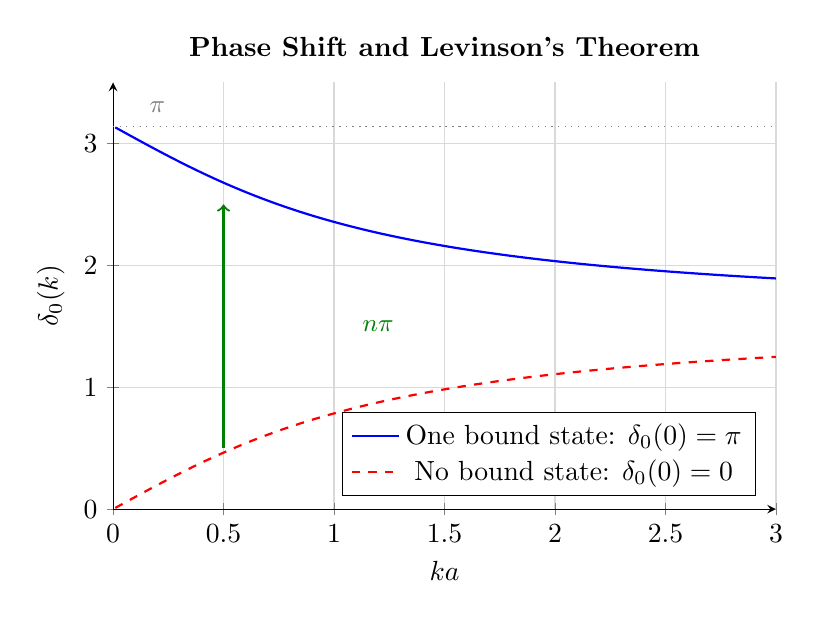
\begin{tikzpicture}
\begin{axis}[
    width=10cm,
    height=7cm,
    xlabel={$ka$},
    ylabel={$\delta_0(k)$},
    title={\textbf{Phase Shift and Levinson's Theorem}},
    xmin=0, xmax=3,
    ymin=0, ymax=3.5,
    axis lines=left,
    grid=major,
    grid style={gray!30},
    samples=200,
    legend pos=south east,
]

% Phase shift with one bound state: delta = pi - arctan(ka)
\addplot[thick,blue,domain=0.01:3] 
    {pi - rad(atan(x*1))};
\addlegendentry{One bound state: $\delta_0(0) = \pi$}

% Phase shift with no bound state: delta = arctan(ka)
\addplot[thick,red,dashed,domain=0.01:3] 
    {rad(atan(x*1))};
\addlegendentry{No bound state: $\delta_0(0) = 0$}

% Pi reference line
\addplot[gray,dotted,domain=0:3] {pi};
\node[gray,font=\small] at (axis cs:0.2,3.3) {$\pi$};

% Arrows showing the difference
\draw[->,thick,green!50!black] (axis cs:0.5,0.5) -- (axis cs:0.5,2.5);
\node[green!50!black,font=\small] at (axis cs:1.2,1.5) {$n\pi$};

\end{axis}
\end{tikzpicture}

\end{document}
